%SOURCE : http://texblog.net/latex-archive/maths/pgf-tikz-commutative-diagram/

% TikZ: chains with labeled edges
% demonstration example
% author: Stefan Kottwitz , http://texblog.net
\documentclass[a4paper,10pt]{article}
\usepackage{tikz}
\usetikzlibrary{arrows,chains,matrix,positioning,scopes}

\makeatletter
\tikzset{join/.code=\tikzset{after node path={%
\ifx\tikzchainprevious\pgfutil@empty\else(\tikzchainprevious)%
edge[every join]#1(\tikzchaincurrent)\fi}}}
\makeatother

\tikzset{>=stealth',every on chain/.append style={join},
         every join/.style={->}}

\begin{document}
\centering

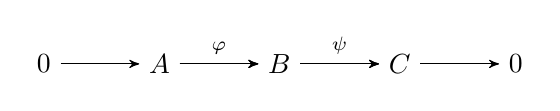
\begin{tikzpicture}[start chain] {
    \node[on chain] {$0$};
    \node[on chain] {$A$} ;
    \node[on chain, join={node[above] {$\scriptstyle\varphi$}}] {$B$};
    \node[on chain, join={node[above] {$\scriptstyle\psi$}}] {$C$};
    \node[on chain] {$0$}; }
\end{tikzpicture}
\bigskip

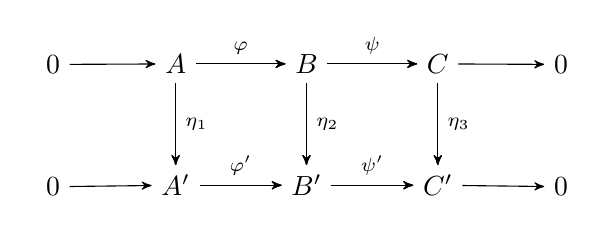
\begin{tikzpicture}
  \matrix (m) [matrix of math nodes, row sep=3em, column sep=3em]
    { 0 & A  & B  & C  & 0 \\
      0 & A' & B' & C' & 0 \\ };
  { [start chain] \chainin (m-1-1);
    \chainin (m-1-2);
    { [start branch=A] \chainin (m-2-2)
        [join={node[right] {$\scriptstyle\eta_1$}}];}
    \chainin (m-1-3) [join={node[above] {$\scriptstyle\varphi$}}];
    { [start branch=B] \chainin (m-2-3)
        [join={node[right] {$\scriptstyle\eta_2$}}];}
    \chainin (m-1-4) [join={node[above] {$\scriptstyle\psi$}}];
    { [start branch=C] \chainin (m-2-4)
        [join={node[right] {$\scriptstyle\eta_3$}}];}
    \chainin (m-1-5); }
  { [start chain] \chainin (m-2-1);
    \chainin (m-2-2);
    \chainin (m-2-3) [join={node[above] {$\scriptstyle\varphi'$}}];
    \chainin (m-2-4) [join={node[above] {$\scriptstyle\psi'$}}];
    \chainin (m-2-5); }
\end{tikzpicture}

\end{document}
